\section{State of the art}
I dette afsnit har vi forsøgt at finde en bred vifte af forskellige løsninger der kan løse et eller flere problemer i forbindelse med indkøb og madlavning, omhandlende indkøbslister, tilbud og opskrifter.

Der vil blive kigget på web services og applikationer, der har til formål at løse nogle af de samme problemer, der berører vores emne.
Løsningerne, der er præsenteret i dette afsnit, forsøger at afhjælpe de problemer beskrevet af de adspurgte i interviewene i \myref{section:interview1}.

\subsection{eTilbudsavis}
eTilbudsavis er en online service, der kan findes på deres hjemmeside\footnote{\underline{www.etilbudsavis.dk}}. eTilbudsavis er en online avis med en høj funktionalitet og en nem brugergrænseflade.
Der kan på siden oprettes et login, således der kan findes tilbage til ændringer på et senere tidspunkt eller andre enheder.
eTilbudsavis har tre mærkbare funktioner, som brugeren har adgang til, hvilket er tilbudsaviser, ønske- og indkøbslister og tilbud.

Tilbudsavis-funktionen, hvilket kan ses på \myref{ss:eTilbudsavis}, indeholder også den mulighed at sætte en præference på, hvor store en radius man vil lede i efter butikkers tilbudsaviser.
Under hver avis, som det ses på figuren, er der også angivet afstand i meter fra ens aktuelle placering.
Der kan vælges imellem alle aviser, som er tilgængelige online og inden for den valgte radius.
Aviserne bliver opdateret løbende, så når der er en ny tilgængelig, bliver den gamle fjernet.
Inde i aviserne kan man trykke på en vare, og den bliver tilføjet til en liste.

\begin{wrapfigure}{o}{0.68\textwidth}
\vspace{-20pt}
	\begin{center}
		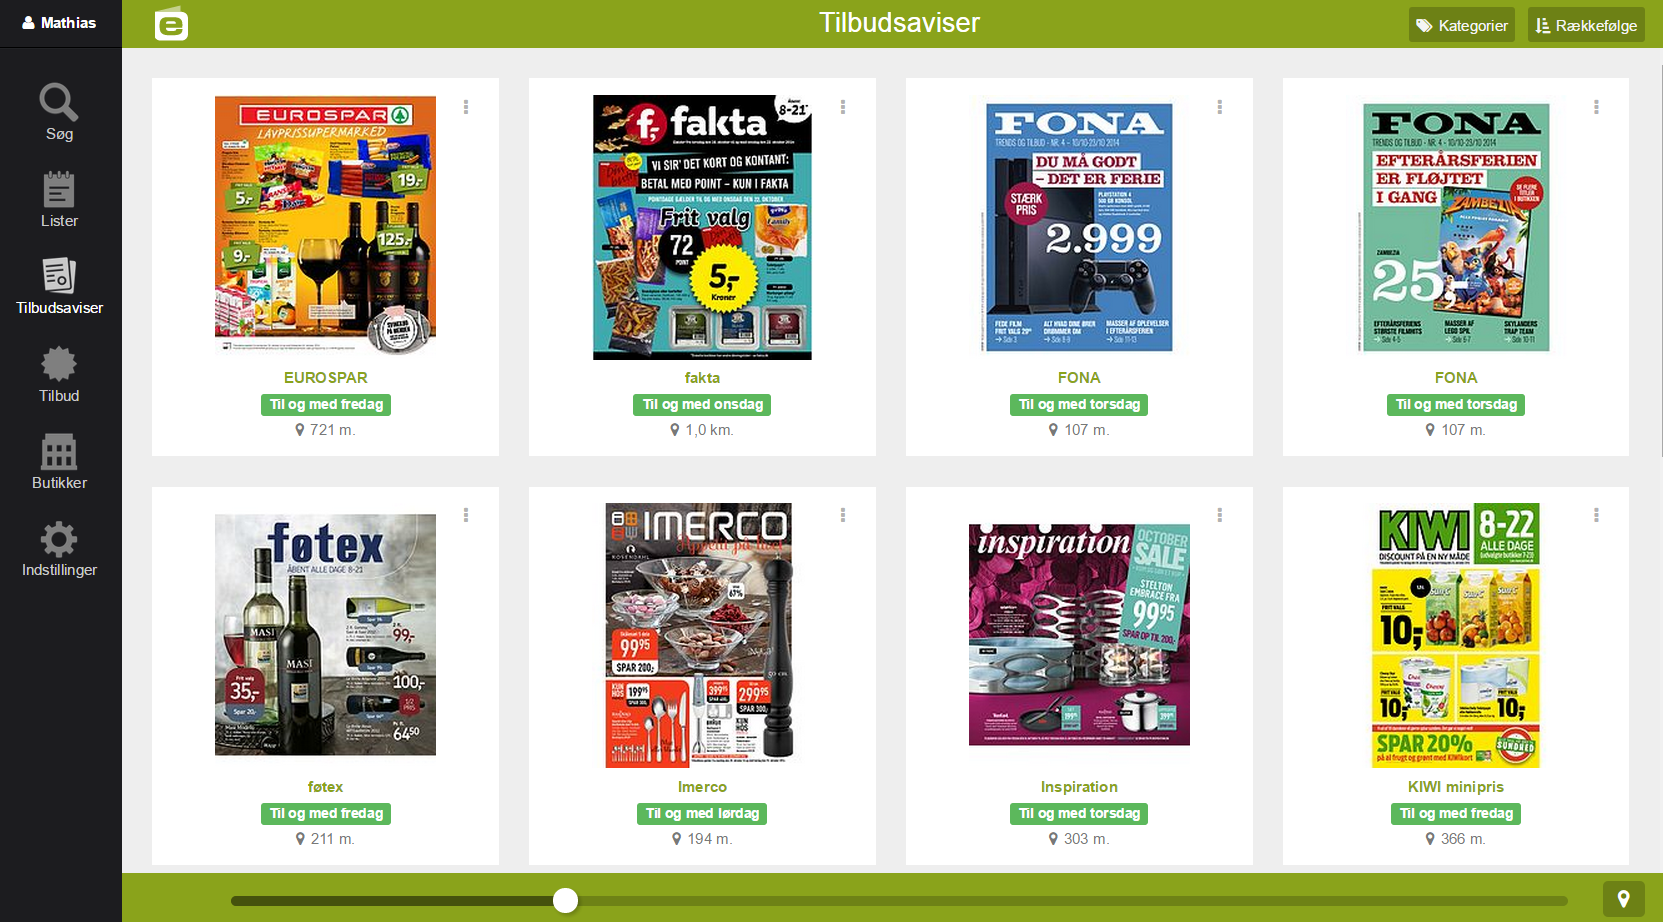
\includegraphics[width=0.66\textwidth]{images/Images/eTilbudsavis.PNG}
	\end{center}
	\vspace{-20pt}
	\caption{Tilbudsaviser på eTilbudsavis.dk}\label{ss:eTilbudsavis}
	\vspace{-20pt}
\end{wrapfigure}

Der er mulighed for at tilføje varer til to lister, en indkøbsliste og en ønskeliste.
Når en vare er valgt, bliver den tilføjet til den valgte liste.
Listen indeholder navn, butik, pris og den valgte mængde, for varen.
Der kan foruden det at vælge varer fra tilbudsaviserne, nemt skrives generiske varer på listen. Varen på listen kan da krydses af for at kunne holde styr på, hvad der er blevet købt.

Hvis der ikke ønskes at skulle bladres tilbudsaviser igennem, er der den mulighed at få vist en hel side kun med tilbud.
Alle aktuelle tilbud fra aviserne, er da vist som elementer med navn, beskrivelse, pris, butik og afstand. Disse tilbud kan på samme måde nemt tilføjes til listerne.

eTilbudsavis er en god online løsning, som har mange gode features, derfor har vi også brugt dem som kilde til vores tilbud gennem deres API.
Dette API er beskrevet i \myref{api}.

\subsection{Tilbudsugen}
Tilbudsugen minder på mange måder om eTilbudsavis, og kan findes på deres hjemmeside\footnote{\underline{www.tilbudsugen.dk}}.
Den har samtlige dagligvareaviser, samt flere inden for bl.a. byggemarkeder, og autoudstyr.
De giver et nemt overblik over diverse aviser, og man kan hurtigt og nemt læse dem på nettet.
Der er desuden mulighed for at lave præferencer som ved eTilbudsavis, her kan man bl.a. vælge økologi eller nøglehulsmærket.
Når man tilføjer en vare til indkøbslisten, søger den automatisk efter tilbud på den valgte vare.
Man bliver bedt om at vælge et specifikt tilbud, og netop dette tilbud bliver tilføjet til indkøbslisten med pris, butik, udløbsdato, mængde og et billede af varen.
Man kan som i eTilbudsavis også trykke på en vare direkte i avisen for at tilføje den til sin liste.
Hvis man vil dele sin indkøbsliste, er det også en mulighed vha. en ``delekode'' som man kan give til en anden bruger - de kan på denne måde også se listen.
Funktionerne findes på hjemmesiden, men det er ikke altid de virker.
For eksempel hvis man tilføjer noget uden at angive et antal, og du så prøver at dele listen med en, vil de ikke være at finde på listen.
Desuden kan man ikke ændre på antallet af varen, du allerede har sat på din indkøbsliste.
For at opnå dette, skal man slette varen, og tilføje den igen med det nye antal.
De har desuden også en smartphone app, men denne crasher ofte, når man benytter sig af deres indkøbsliste, men fungerer tilgengæld fint, hvis man blot vil se på ugens tilbud i aviserne.

Tilbudsugen er et lidt dårligere alternativt til eTilbudsavis, da der er problemer med delbarheden af indkøbslisterne, samt den app, der er stillet til rådighed, ikke er stabil.
Derimod er den nem at navigere, siden er brugervenlig og ser overskuelig ud.

\subsection{Smartphone Apps udgivet af butikker}
På \myref{tbl-smartphone} ses der nogle butikskæder, som har udviklet android apps, samt hvilke funktionaliteter disse har.
For at skabe et overblik, er der udvalgt features, og disse er blevet opsat i et skema for overskuelighedens skyld.
\begin{table}[H]
	\centering
		\colorlet{shadecolor}{gray!40}
    	\rowcolors{1}{white}{shadecolor}
	    \begin{tabular}{l|lllllllllll}
	    %Table: http://bit.ly/1tD6EI6
	   	%Funktionalitet & Tilbudsavis & Indkøbsliste & Opskrifter & Varescan & Find butik & Budget & Madplan & Rabatkupon/fordelsordning & Deling af indkøbslister & Rating på Play & Senest opdateret \\ \hline
	     & \rot{Tilbudsavis} & \rot{Indkøbsliste} & \rot{Opskrifter} & \rot{Varescan} & \rot{Find butik } & \rot{Budget} & \rot{Madplan} & \rot{Rabatkupon} & \rot{Deling} & \rot{Play rating} & \rot{Senest} \rot{opdateret} \\ \hline
	   	Føtex                       & \cmark   & \cmark    & \cmark  & \cmark   & \cmark  & ~      & ~       & ~          & ~                       & 3.4 (354)      & 2014-07-24       \\
	    SPAR                        & \cmark   & \cmark    & \cmark  & ~        & \cmark  & \cmark & ~       & ~          & ~                       & 2.8 (64)       & 2014-05-15       \\
	    Fakta                       & \cmark   & \cmark    & \cmark  & ~        & \cmark  & ~      & \cmark        & \cmark     & \cmark               & 3.1 (454)      & 2014-08-02       \\
	    FaktaQ                      & \cmark   & ~         & \cmark  & ~        & \cmark  & ~      & ~       & ~          & ~                       & 4.4 (7)        & 2014-03-11       \\
	    REMA 1000                   & \cmark   & \cmark    & \cmark  & ~        & \cmark  & ~      & ~       & ~          & ~                       & 3.5 (674)      & 2014-04-16       \\
	    SuperBrugsen                & \cmark   & \cmark    & \cmark  & ~        & \cmark  & ~      & ~       & ~          & ~                       & 3.8 (987)      & 2014-06-30       \\
	    Kvickly                     & \cmark   & \cmark    & \cmark  & ~        & \cmark  & ~      & ~       & ~          & ~                       & 3.7 (632)      & 2014-07-20       \\
	    \end{tabular}
	    \caption{Nogle butikskæder med smartphone apps samt deres funktionaliteter.}\label{tbl-smartphone}
	\end{table}
Vi har valgt at undersøge en af disse apps nærmere, og valget faldt på Faktas app, MitFakta, da denne bliver opdateret og har flest funktioner.
\subsubsection{Faktas Android App}

\begin{wrapfigure}{o}{0.4\textwidth}
\vspace{-20pt}
	\begin{center}
		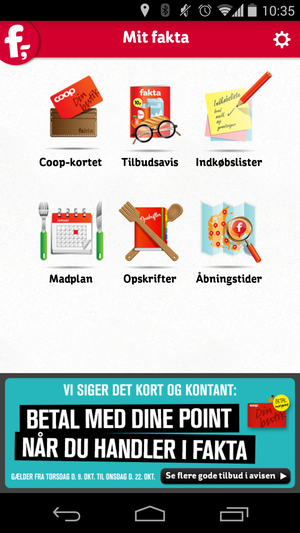
\includegraphics[width=0.38\textwidth]{images/Images/MitFakta.png}
	\end{center}
	\vspace{-20pt}
	\caption{MitFakta}
	\vspace{-20pt}
	\label{ss:MitFakta}
\end{wrapfigure}

Faktas android app kalder de for ``Mit fakta'', den er som helhed overskuelig.
Efter åbning af appen kan man vælge mellem seks menupunkter eller ændre sine indstillinger, disse kan ses på \myref{ss:MitFakta}.
Første menupunkt omhandler ``Coop-kortet'', og giver brugeren mulighed for at indtaste sine medlemsinfomationer, da disse giver særlige tilbud.
Andet menupunkt er deres tilbudsavis, hvilket er en digital kopi af den fysiske tilbudsavis.
Dog kan man fra den også tilføje varer til sin indkøbsliste, eller se varerne i et gitterformat.
Tredje menupunkt er ``indkøbsliste'', her kan man have flere personlige og/eller delte indkøbslister.
Her kommer deres Facebook integration også i spil, som tillader nem deling af indkøbslister med brugerens Facebook venner.
Fjerde menupunkt er en madplan, hvori man kan planlægge sin egen madplan, eller se Faktas anbefalinger til en ``under 20 kr pr. person pr. aften''-løsning.
Femte menupunkt er deres opskrifter.
Her findes der et stort antal af opskrifter, disse kan tilføjes direkte til ens madplan eller indkøbslister (både personlige og delte).
Sjette menupunkt hedder ``Åbningstider'', og her kan brugeren finde Faktas butikker samt deres forskellige åbningstider.

Appen virker rigtigt godt, der er ingen blindgyder, og derfor er den meget nem at navigere rundt i. Der er lagt meget fokus på den sociale del, da der kan deles med venner på facebook, hvilket simplificerer delingen af indkøbslister. Den eneste ulempe, der er ved denne app, er, at den kun er egnet til vare fra Fakta, og derfor sætter en del restriktioner på sig selv.

\subsection{Tøm køleskabet}
Der findes talrige tjenester, der tilbyder ``at tømme dit køleskab''.
Mere specifikt, tilbyder de en service, hvor du som bruger, angiver hvilke varer dit køleskab pt. indeholder, samt hvilke andre ingredienser du har til rådighed.
Derefter får du så præsenteret en række forskellige opskrifter, der kan laves ud fra dine tilgængelige ingredienser.
De fleste af tjenesterne (herunder dem vi her har undersøgt) viser også opskrifter, som indeholder yderligere ingredienser.
Dette betyder naturligvis, at man som bruger ikke bliver fritaget fra at handle ind, hvis man mangler nogle ingredienser til lige netop den opskrift, man vælger at udføre.
Tjenesten \textit{MyFridgeFood} \footnote{\underline{www.myfridgefood.com}} tilbyder at oprette en indkøbsliste ud fra netop disse manglende ingredienser, hvilket kan lade sig gøre blandt andet fordi, alle opskrifter er interne på \textit{MyFridgeFood}.
I modsætning til dette er der \textit{Supercook} \footnote{\underline{www.supercook.com}}, som linker til eksterne opskrifter, og ikke tilbyder at generere en indkøbsliste.
Umiddelbart anbefales opskrifter ikke ud fra den enkelte brugers smag og madvaner, men udelukkende på baggrund af, hvad man ``har i køleskabet''.
Grundet dette virker tjenesterne mere som simple filtreringer af databaseopslag, end egentlige anbefalinger, der tager højde for brugerens smag og præferencer indenfor den gastronomiske verden.

\subsection{Alternativer til Indkøbsturen}
Der findes altså allerede mange applikationer, i form af apps til smartphones og webapps, som kan hjælpe med indkøbsturen og planlægning af måltider.
Hvis disse indeholder opskrifter, som tager højde for tilbudene i en given uge, er det inden for en enkelt butikskædes tilbud.
Der er altså ingen applikationer, der tager højde for tilbud fra alle butikskæderne.
I dette afsnit undersøges alternativer til indkøbsturen.

Ud over mobilapplikationer, flytter nogle dagligvarebutikker på internettet, sådan man kan handle ind hjemmefra, som man kender det fra almindelig nethandel.
Andre løsninger er baseret på abonnementsordninger, som fjerner meget af planlægningen fra ordningens bruger.
Herunder gennemgås eksempler på nogle firmaer, der tilbyder de to ovennævnte løsninger.

De seneste år har online dagligvare-butikker skudt frem, og selvom de er i kraftig vækst udgør de kun en lille del af det samlede dagligvareforbrug i Danmark\citep{SOTA_MP1}.

\subsubsection{Online butikker}
Eksempler på online dagligvarebutikker er SuperBest\footnote{\underline{www.superbest.dk}} og Irma\footnote{\underline{www.irma.dk}}
Nogle af butikkerne har dog kun en online butik, og ingen fysisk modpart, dette er butikker som Nemlig.com\footnote{\underline{www.nemlig.com}} og Osuma\footnote{\underline{www.Osuma.dk}}.
Disse butikker kan gøre det lettere at handle ind.
Sådanne butikker giver både mulighed for at handle ind hjemmefra, fra studiet eller fra arbejdet i en pause.
Ved at handle hjemmefra kan man også let overskue, hvad man mangler, imens man handler ind, og man kan derfor undgå at glemme at skrive noget på indkøbssedlen.
Ligeledes undgår man at stå i supermarkedet og være i tvivl om, man mangler en bestemt vare.
Nogle af firmaerne tilbyder også opskrifter.
Nemlig.com tilbyder opskrifter, og hjemmesiden kan præsentere alle deres varer, som indgår i listen over ingredienser.
Dette gør, at man direkte fra en given opskrift, kan sammenligne tilsvarende varer og tilføje en af dem til sin indkøbskurv.
Andre butikker giver også mulighed for at oprette madplaner, hvilket kan gøre planlægningen af indkøb og madlavning i hjemmet lettere.
Disse online butikker kommer dog også med forskellige ulemper i forhold til fysiske supermarkeder.
Det koster penge at få leveret sine varer fra disse butikker, typisk omkring 50 kr., og i nogle af butikkerne skal man købe for et minimumsbeløb.
Ved handel gennem online butikkerne, kan du ikke få varerne med det samme; det varierer butikkerne imellem, hvor stor ventetiden er.
Disse to ulemper gør ligeledes, at man ikke kan benytte disse løsninger, hvis man står og mangler en vare eller to.

\subsubsection{Abonnementsordninger}
Ordningerne sender typisk kasser med daglivarer ud til deres kunder.
Disse kassers indhold tilbyder ofte en varieret blanding af kød, grønt og frugt.
I denne kategori findes udbydere som Aarstiderne og igen SuperBest\citep{SOTA_MP_AAR, SOTA_MP_SB}.
Ideen med sådanne kasser er, at nogle ansatte, typisk kokke eller lignende ved eksempelvis Aarstiderne, har sammensat kasser med ingredienser til mellem tre og fem aftensmåltider.
På deres hjemmeside eller mobilappikation kan man så finde guider og opskifter til, hvordan maden tilberedes.
Derudover har Aarstiderne også suppleret med ydeligere tre kategorier, for at de kan tilbyde mere fleksible løsninger til kunderne.
Den første kategori holder sig inde for kasse-dogmet og er generelle kasser, hvor man eksempelvis kan købe en kødkasse, fiskekasse eller en frugtkasse; i disse kategorier findes der så forskellige kasser inden for hver kategori.
Anden kategori er supplering, hvorigennem kunderne kan købe forskellige varer i løssalg, hvis ikke kasserne opfylder deres behov.
Sidste kategori er morgenmad, her tilbyder de en blanding mellem kasser og løssalg.
Denne model kan løse mange problemer i forhold til madlavningen for kunderne.
Løsningen vil kunne mindske den planlægning en person behøves foretage sig, fordi kasserne indeholder alle ingredienser til flere måltider, samt opskrifter at følge.
Dette betyder, at kunden hverken behøves planlægge aftensmaden eller indkøbet dertil.
Ligeledes ville den kraftigt mindske behovet for at handle ind andre steder.
Denne løsning kommer dog heller ikke uden ulemper.
Dogmet med at forudbestemme flere måltider og have de eksakte ingredienser, begrænser den kreativitet, som en person normalt ville kunne udleve i køkkenet.
Ydermere begrænses ideen meget af den moderne families struktur, hvor det ofte ikke er hele familien, der spiser sammen mange dage om ugen.
Det er også svært at tage højde for præferencer som kræsenhed eller allergier i disse forudbestemte kasser.
Denne løsning vil heller ikke kunne fritage en bruger fra at skulle handle ind andre steder end her, da de ikke tilbyder alt.

Som vi har set i ovenstående gennemgang, findes der alternativer til den klassiske indkøbstur, der er dog ingen af disse, der formår at løse alle problemerne.
Ved alle løsningerne opstår også nye ulemper og problemstillinger i forhold til almindeligt indkøb.
Alt taget i betragtning vil det komme meget an på nuværende vaner og familiestrukturen, om disse muligheder vil være en god løsning for en given familie.


\fxnote{Strukturen her med subsubsections, ligner lort :D AAALt for mange tal.}